\section{Feedforward neural network}
Feedforward neural network is a network whether unit in the graph does not form a cycle \cite{Goodfelloetal2016}. 

Each feedforward neural network consist at least one input layer, one output layer. Each layer contain one or more neurons (network nodes). Each neuron consist of a linear activation or non-linear activation function. 

Each node have an activation function. There are two type of activation function: Linear and non-linear. 

Example of linear function: \\
\[f(x) = Wx + b \]

Example of non-linear function: \\
\[f(x) = tanh(x) \]
\[f(x) =\frac{1}{1+e^{-x}} \]

\subsection{Single-layer perceptron}
Singlelayer perceptron is a feedforward neural network only have one input layer and one output layer of neuron unit (See fig \ref{fig:singleperceptron}). Singlelayer perceptron cannot solve some problem such as XOR.
\begin{figure}[H]
	\centering
	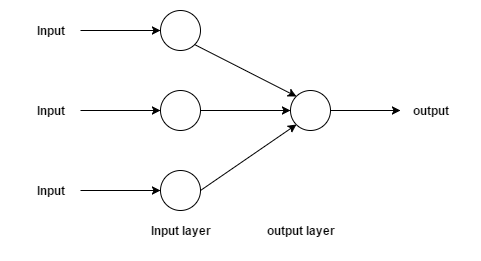
\includegraphics[width=0.7\linewidth]{figure/singleperceptron}
	\caption[Single-layer Perceptron]{Single-layer Perceptron}
	\label{fig:singleperceptron}
\end{figure}



\subsection{Multi-layer perceptron}
Multilayer perceptron (MLP) is a feedforward neural network consist of 2 or more layer (See fig \ref{fig:multilayerperceptron}). First layer called input layer. Last layer called output layer. All layer between input and output layer are hidden layer. A series of linear function is equal to 2 layer perceptron. Hence, MLP always contain non-linear activation function. In MLP, every unit of previous layer connect to all unit in next layer.

\begin{figure}[H]
	\centering
	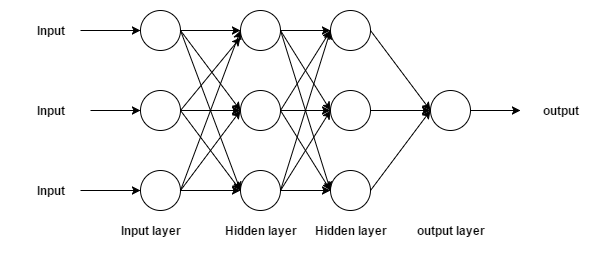
\includegraphics[width=0.7\linewidth]{figure/multilayerperceptron}
	\caption[Multi-layer Perceptron]{Multi-layer Perceptron}
	\label{fig:multilayerperceptron}
\end{figure}

\subsection{Forward pass}
Forward pass, or forward propagation, is a process which information from input x flow through the network to output y. In MLP forward pass, an input x is feed through first layer, also known as input layer. Output from first layer is use as input for second layer, and so on until it reach last layer, output layer. Output from output layer are output of MLP. 

For example: a MLP with 4 activation function: $f(x)$, $g(x)$, $h(x)$, $k(x)$. With $f(x)$ is input layer, $k(x)$ is output layer, and $g(x), h(x)$ are hidden layers .With input $x$, then MLP has output $ y = k(h(g(f(x))))$.

\subsection{Cost function}
Cost function $J(\theta)$  is a measurement how far predicted  $\hat y$ from expected label $y$. When our model predict exactly the labeled output, then cost function is zero. The problem is to minimize the cost function. Cost function of MLP dependent on output layer.

For most of our experiment, we would use softmax output layer and cross-entropy loss function.
\subsection{Backward pass}



